\chapter{مدل‌سازی پخش‌اطلاعات در شبکه‌های اجتماعی آنلاین}
\newpage
\begin{persian}
\section {مقدمه}
\noindent
در این فصل به معرفی مدل‌های مطرح شده برای فرایند پخش اطلاعات خواهیم پرداخت. در ادامه توضیحی مختصر برای تک تک این مدل‌ها به همراه‌یک طبقه بندی براساس خصوصیات مدل‌های مورد نظر ارایه شده است. سرانجام مدل‌های معرفی شده را مقایسه می‌کنیم و سرانجام هم ارجاع‌های لازم برای مطالعه بیشتر برای انواع مدل‌های مشتق شده از مدل‌های اولیه و اصلی داده خواهند شد. ضمنا در این فصل کلمات گره و رأس و همین‌طور یال و اتصال دو به دو مترادف هم می‌باشند.
%\newpage
\section {مدل‌های پخش اطلاعات}
\noindent
در گذشته از مدل‌های همه گیری مریضی‌های مسری مانند سل برای مدل سازی فرایند پخش اطلاعات در سطح شبکه‌های اجتماعی استفاده شده است \cite{watts_six_2004,easley_networks_2010}. در سال‌های اخیر مدل‌های مانند مدل انتشار مستقل\پانویس{\lr{ Independent Cascading Model}} 
و مدل آستانه خطی\پانویس {\lr{ Linear Threshold Model}}
در زمینه بررسی الگوریتمیک فرایند پخش به این دسته از مدل‌ها اضافه شده اند. دو مدل \lr{LT} و \lr{IC} به صورت امروزی نخستین بار در \cite {kempe_maximizing_2003} برای بررسی مسئله‌ی حداکثر سازی تاثیر اجتماعی افراد یک شبکه‌ی اجتماعی برای پذیرفتن و ترویج نوآوری پیشنهاد شده اند.
این دو مدل و همین‌طور مدل‌های همه گیری جزو مدل‌های اصلی فرایند پخش اطلاعات می‌باشند که مشتقات زیادی برای آنان ارایه شده است. هم چنین مدل‌هایی براساس نظریه بازی‌ها\پانویس {\lr{ Game Theoric Models}} \cite{jiang_evolutionary_2013} و همین طور مدل‌هایی بر پایه زنجیره‌های مارکوف پیوسته زمان برای مدل سازی و بررسی فرایند پخش اطلاعات پیشنهاد شده اند، که در بخش پایانی این فصل ارجاع‌های مربوط به این مدل‌ها برای مطالعه‌ی بیشتر خواننده داده شده است. 
\\


%\newpage
\section{مدل‌های انتشار}
\noindent
{
در این بخش به معرفی و تشریح مدل‌های انتشار مطرح برای مدل‌کردن فرایند پخش اطلاعات می‌پردازیم. 
}
\subsection{مدل انتشار مستقل}
\noindent
{
مدل انتشار مستقل جزو دو مدل اصلی و مطرح برای مدل‌سازی فرایند پخش اطلاعات در سطح شبکه‌های اجتماعی است. ریشه‌ی این مدل به مدل‌های حرکت ذرات در فیزیک باز می‌گردد \cite{chen_scalable_2010}. به طور کلی این مدل و مشتقات آن‌ها برای مدل سازی پذیرش و استفاده‌ی چیز‌های جدید و تاثیرگذار در بستر شبکه‌های اجتماعی به کار رفته شده اند. در این مدل بستر پخش اطلاعات یک گراف جهت‌دار ایستا $G =(V,E)$ در نظر گرفته می‌شود که $V$ و $E$ به ترتیب مجموعه‌های گره‌ها و یال‌های $G$ می‌باشند. هر اتصال یعنی وجود یک یال جهت دار از گره $n$ به گره $x$ در این شبکه به صورت $e=(n,x)$ که $n \neq x$ تعریف می‌شود.
برای هر گره‌ مانند $n$ مجموعه‌ی فرزندان $n$ یا $C_n$ به صورت $C_n = \{x; x \in (n,x)\}$ تعریف می‌شود و همین‌طور تابع والدین $n$ هم به نام $H_n$ به صورت $W_n =\{x; x \in (x,n)\}$ تعریف می‌شود. \\
\indent
در این مدل در ابتدا به هر یال جهت دار $e$ عدد مثبت $p_{nx}$ با شرط $0 < p_{nx} < 1$ نسبت داده می‌شود. به $p_{nx} $ احتمال پخش $(n,x)$ هم گفته می‌شود. فرایند پخش با انتخاب یک مجموعه‌ی آغازین به نام $D(0)$ از گره‌های شبکه‌ی مورد مطالعه شروع می‌شود، بدین صورت که با فرض این امر که در اینجا نیز هر گره می‌تواند در یکی از دو حالت فعال و یا غیر فعال باشد، گره‌هایی که در $D(0)$ قرار دارند در حالت فعال فرض می‌شوند و در هر گام زمانی $t=\{0,1,..,w\}$ یک گره فعال مانند ‌$n$ می‌تواند هر گره فرزند غیر فعال خود مانند $x$ را با احتمال $p_{nx}$ فعال کند. باید توجه داشت در صورتی که چند گره والد گره‌ای مانند $n$ در گام $t$ فعال باشند ترتیب اعمال احتمال فعال سازی $n$ توسط یکی از آن‌ها به صورت اختیاری و بدون در نظر گرفتن اولویت خاصی در نظر گرفته می‌شود و تنها امر مهم این است که فعال سازی برای $n$ از طرف گره‌های والدش باید همگی در گام $t$ انجام پذیرد. ضمنا در این مدل جدا از فعال شدن و یا فعال نشدن گره فرزند در گام $t$ هر گره والد تنها یک بار فرصت فعال سازی گره فرزند خود را دارد. اجرای فرایند انتشار مستقل وقتی دیگر گره‌ای را نتوان 
فعال کرد خاتمه می‌یابد.
در زیر تابع فعال سازی و مجموعه‌ی $\theta$ برای یال دلخواه $e$ را مشاهده می‌کنید.

\centerline{
\scalebox{1.25}{
 \begin{latin}
 $ Y_1(e_i) = p_{e_i} ; \theta =\{p_{nx}; (n,x) \in E\} $
 \end{latin}}}

به کمک مجموعه‌ی $\theta$ می‌توان تابع درجه تأثیر گذاری هر گره‌ یا تعداد گره‌های فرزند گره مورد بحث را که احتمال می‌دهیم در گام بعدی فعال باشند به صورت زیر تعریف کرد.

\centerline{
\scalebox{1.25}{
 \begin{latin}
 $ Y_2(n)=\mu(n,\theta)$
 \end{latin}}}

در اینجا یکی از موارد مهم یافتن آن دسته از گره‌های فعال اولیه خواهد بود(به طور دقیق‌تر $k$ تا گره) که با انتخاب به عنوان مجموعه‌ی گره‌های فعال اولیه، حداکثر پخش اطلاعات را با استفاده از این مدل حاصل می‌آورند. اگر بخواهیم$\mu(n,\theta_0)$ را برای رتبه بندی گره‌ها برای امر ذکر شده محاسبه کنیم، با فرض اینکه$\theta_0$ نشاندهنده‌ی مجموعه‌ی واقعی احتمال‌های پخش برای کل شبکه‌ی ما می‌باشد چون مجموعه‌ی $\theta_0$ را نمی‌توان در اکثر اوقات پیدا کرد می‌توان به‌جای $\mu(n,\theta_0)$ میزان $\mu(n,\hat{\theta})$ را برای گره‌های اولیه محاسبه برای رتبه دهی گره‌ها از نظر تأثیر گذاری روی فرایند پخش اطلاعات محاسبه نمود. در اینجا $\hat{\theta}$ مجموعه احتمالاتی است که به صورت تجربی و تقریبی برای گره $n$ پیدا شده است.



 \begin{figure}[H]
 \centering
 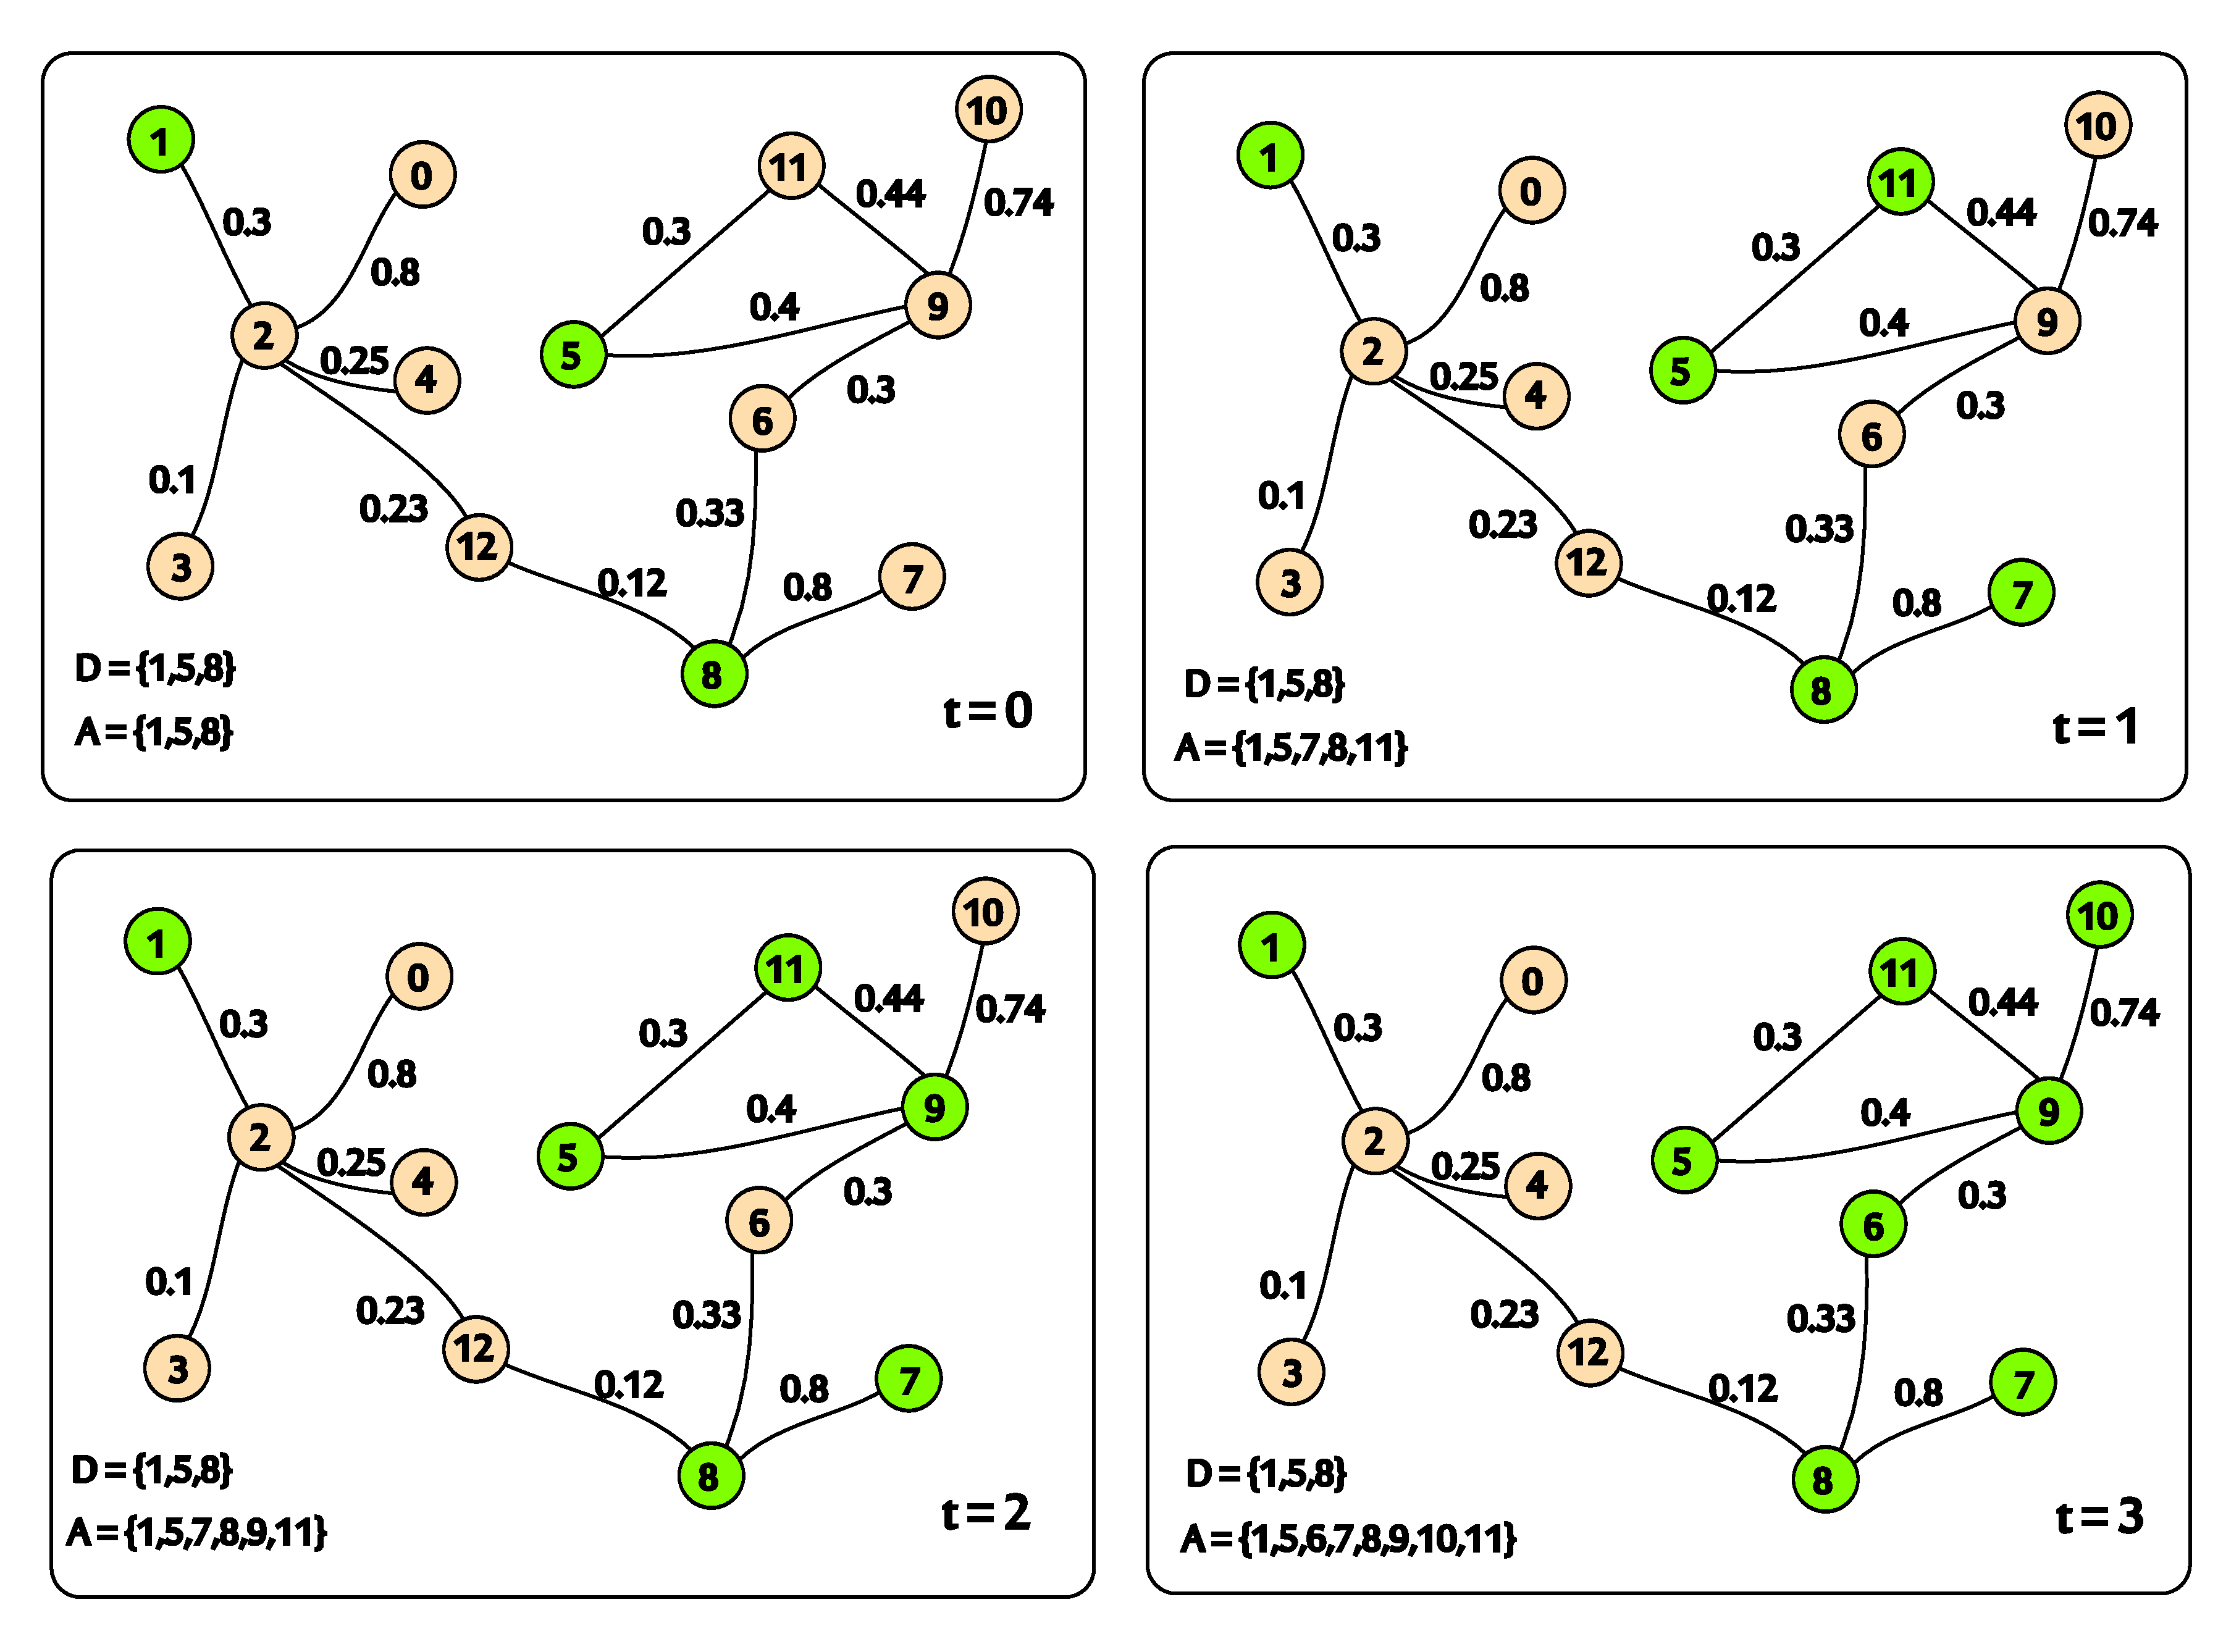
\includegraphics[scale=0.24]{figures/icm}
 \caption[مدل انتشار مستقل]
 { شبیه سازی فرایند کار مدل انتشار مستقل با ۳ گره فعال اولیه.}
\end{figure}

 \begin{figure}[H]
 \centering
 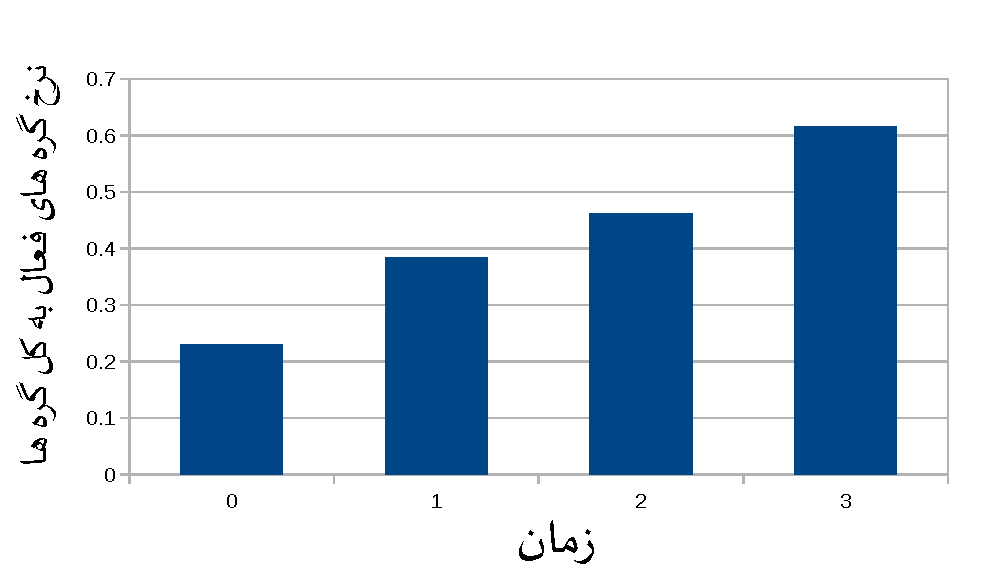
\includegraphics[scale=0.6]{figures/icm_chart1}
 \caption[شبیه سازی مدل انتشار مستقل]
 {روند پخش در حین شبیه سازی فرایند کار مدل انتشار بالا.}
\end{figure}


}

\subsection{مدل انتشار کاهشی}
\noindent{
 مدل انتشار کاهشی\پانویس { Decreasing Cascade Model} در مقایسه با مدل انتشار مستقل عملی تر و عمومی تر می‌باشد. در این مدل اگر $S$ نشان دهنده‌ی مجموعه‌ی گره‌هایی باشد که در گذشته سعی در فعال سازی گره $v$ نموده اند ولی موفق به این کار نشده اند باشد و هم چنین $p_{v}(u|S)$ نشاندهنده‌ی احتمال فعال سازی $v$ توسط $u$ باشد وقتی $S \subset T $ در این مدل $p_{v}(u|T) \geqslant p_{v}(u|S)$ خواهد بود. به زبان ساده تر در این مدل احتمال فعال سازی گره‌هایی که در زمان گذشته تلاش برای فعال سازیشان با شکست روبه رو شده باشد کاهش می‌یابد که با نتایج به دست آمده در دنیای واقعی تطابق دارد.
}

%\newpage
\section{مدل‌های آستانه}
\noindent
{
در این بخش به معرفی و تشریح مدل‌های خانواده‌ی آستانه که برای مدل‌کردن فرایند پخش اطلاعات ارایه شده اند می‌پردازیم. 
}



\subsection{مدل آستانه خطی}
\noindent{
 مدل آستانه اولین بار برای مدل سازی رفتار جمعی افراد یک جامعه توسط مارک گرانووتر در سال ۱۹۷۸ مطرح شده است \cite {granovetter_threshold_1978}. این مدل و مدل‌های مشتق شده از آن برای مدل سازی تأثیر همسایگان در یک شبکه‌ی اجتماعی بر رفتار اعضا و پیش بینی تاثیر پذیری اعضا از هم برای مقاصدی چون تبلیغات به کار گرفته شده اند \cite {chen_scalable_2010}. فکر اصلی این مدل از نظریه‌های جامعه شناسی گرفته شده است و فرض را بر این می‌گذارد که خیلی از چیز‌ها مانند خرید یک کالای جدید و یا شنیدن خبری تازه توسط یک فرد تحت تاثیر کردار همسایگانش در یک اجتماع است. به طور دقیق تر در مدل آستانه خطی مجموعه‌ی $V =\{1,..,n\}$ متشکل از گره‌های(افراد) گراف شبکه‌ی اجتماعی مورد مطالعه به صورت $G =(V,E)$ مفروض است. در اینجا هم مانند مدل انتشار مستقل مجموعه‌ی $E$ نشان دهنده‌ی یال‌های گراف $G$ می‌باشد که گرافی ایستا و جهت دار و بدون طوقه است. مجموعه‌ی همسایگان یک گره در $G$ در این مدل به صورت $N_n = \{n; (n,x) \in E\}$ تعریف می‌شود که معادل مجموعه‌ی فرزندان برای مدل انتشار مستقل می‌باشد و به زبان ساده شامل گره‌هایست که می‌توانند به طور مستقیم 
تحت تأثیر گره $n$ قرار گیرند.\\
در این مدل در لحظه‌ی $t=0$ مانند مدل انتشار مستقل زیرمجموعه‌ای از $V$ به حالت فعال در می‌آید، به طور دقیق این مجموعه‌ی فعالان آغازین را به صورت زیر تعریف می‌کنیم:

\centerline{
\scalebox{1.25}{
\begin{latin}
 $ \Phi(0) \in E $
\end{latin}}}


حال در هر گام $t=\{1,2,..,z\}$ گره غیر فعال $n$ که $n \in V$ در صورتی که حداقل $\phi_n \in (0,1]$ از همسایگانش نیز فعال باشند فعال می‌شود. برای مثال $i$ در گام $t=1$ فعال می‌باشد اگر شرایط زیر در گام $t=0$ برقرار بوده باشد.

\centerline{
\scalebox{1.25}{
\begin{latin}
 $ {{{|\Phi(0) \cap N_i|} \over|N_i|} \geqslant \phi_i} \Rightarrow i \in \Phi(1) $
\end{latin}}}

به زبان دیگر $\Phi(1)$ مجموعه‌ای از افراد شبکه‌ی اجتماعی مورد مطالعه می‌باشد که اطلاعات را از طریق همسایگان خود در گام زمانی $t=0$ دریافت نموده اند. برای گام‌های بالاتر یعنی $t \geqslant 0$ می‌تواند فرایند فعال سازی گره غیر فعال $i$ را به صورت زیر نشان داد.

\centerline{
\scalebox{1.25}{
\begin{latin}
 $ {{{|\{\bigcap_{l=0}^{t-1}\Phi(l)\} \cap N_i|} \over|N_i|} 
 \geqslant \phi_i} \Rightarrow i \in \Phi(k) $
\end{latin}}}
}

 \begin{figure}[H]
 \centering
 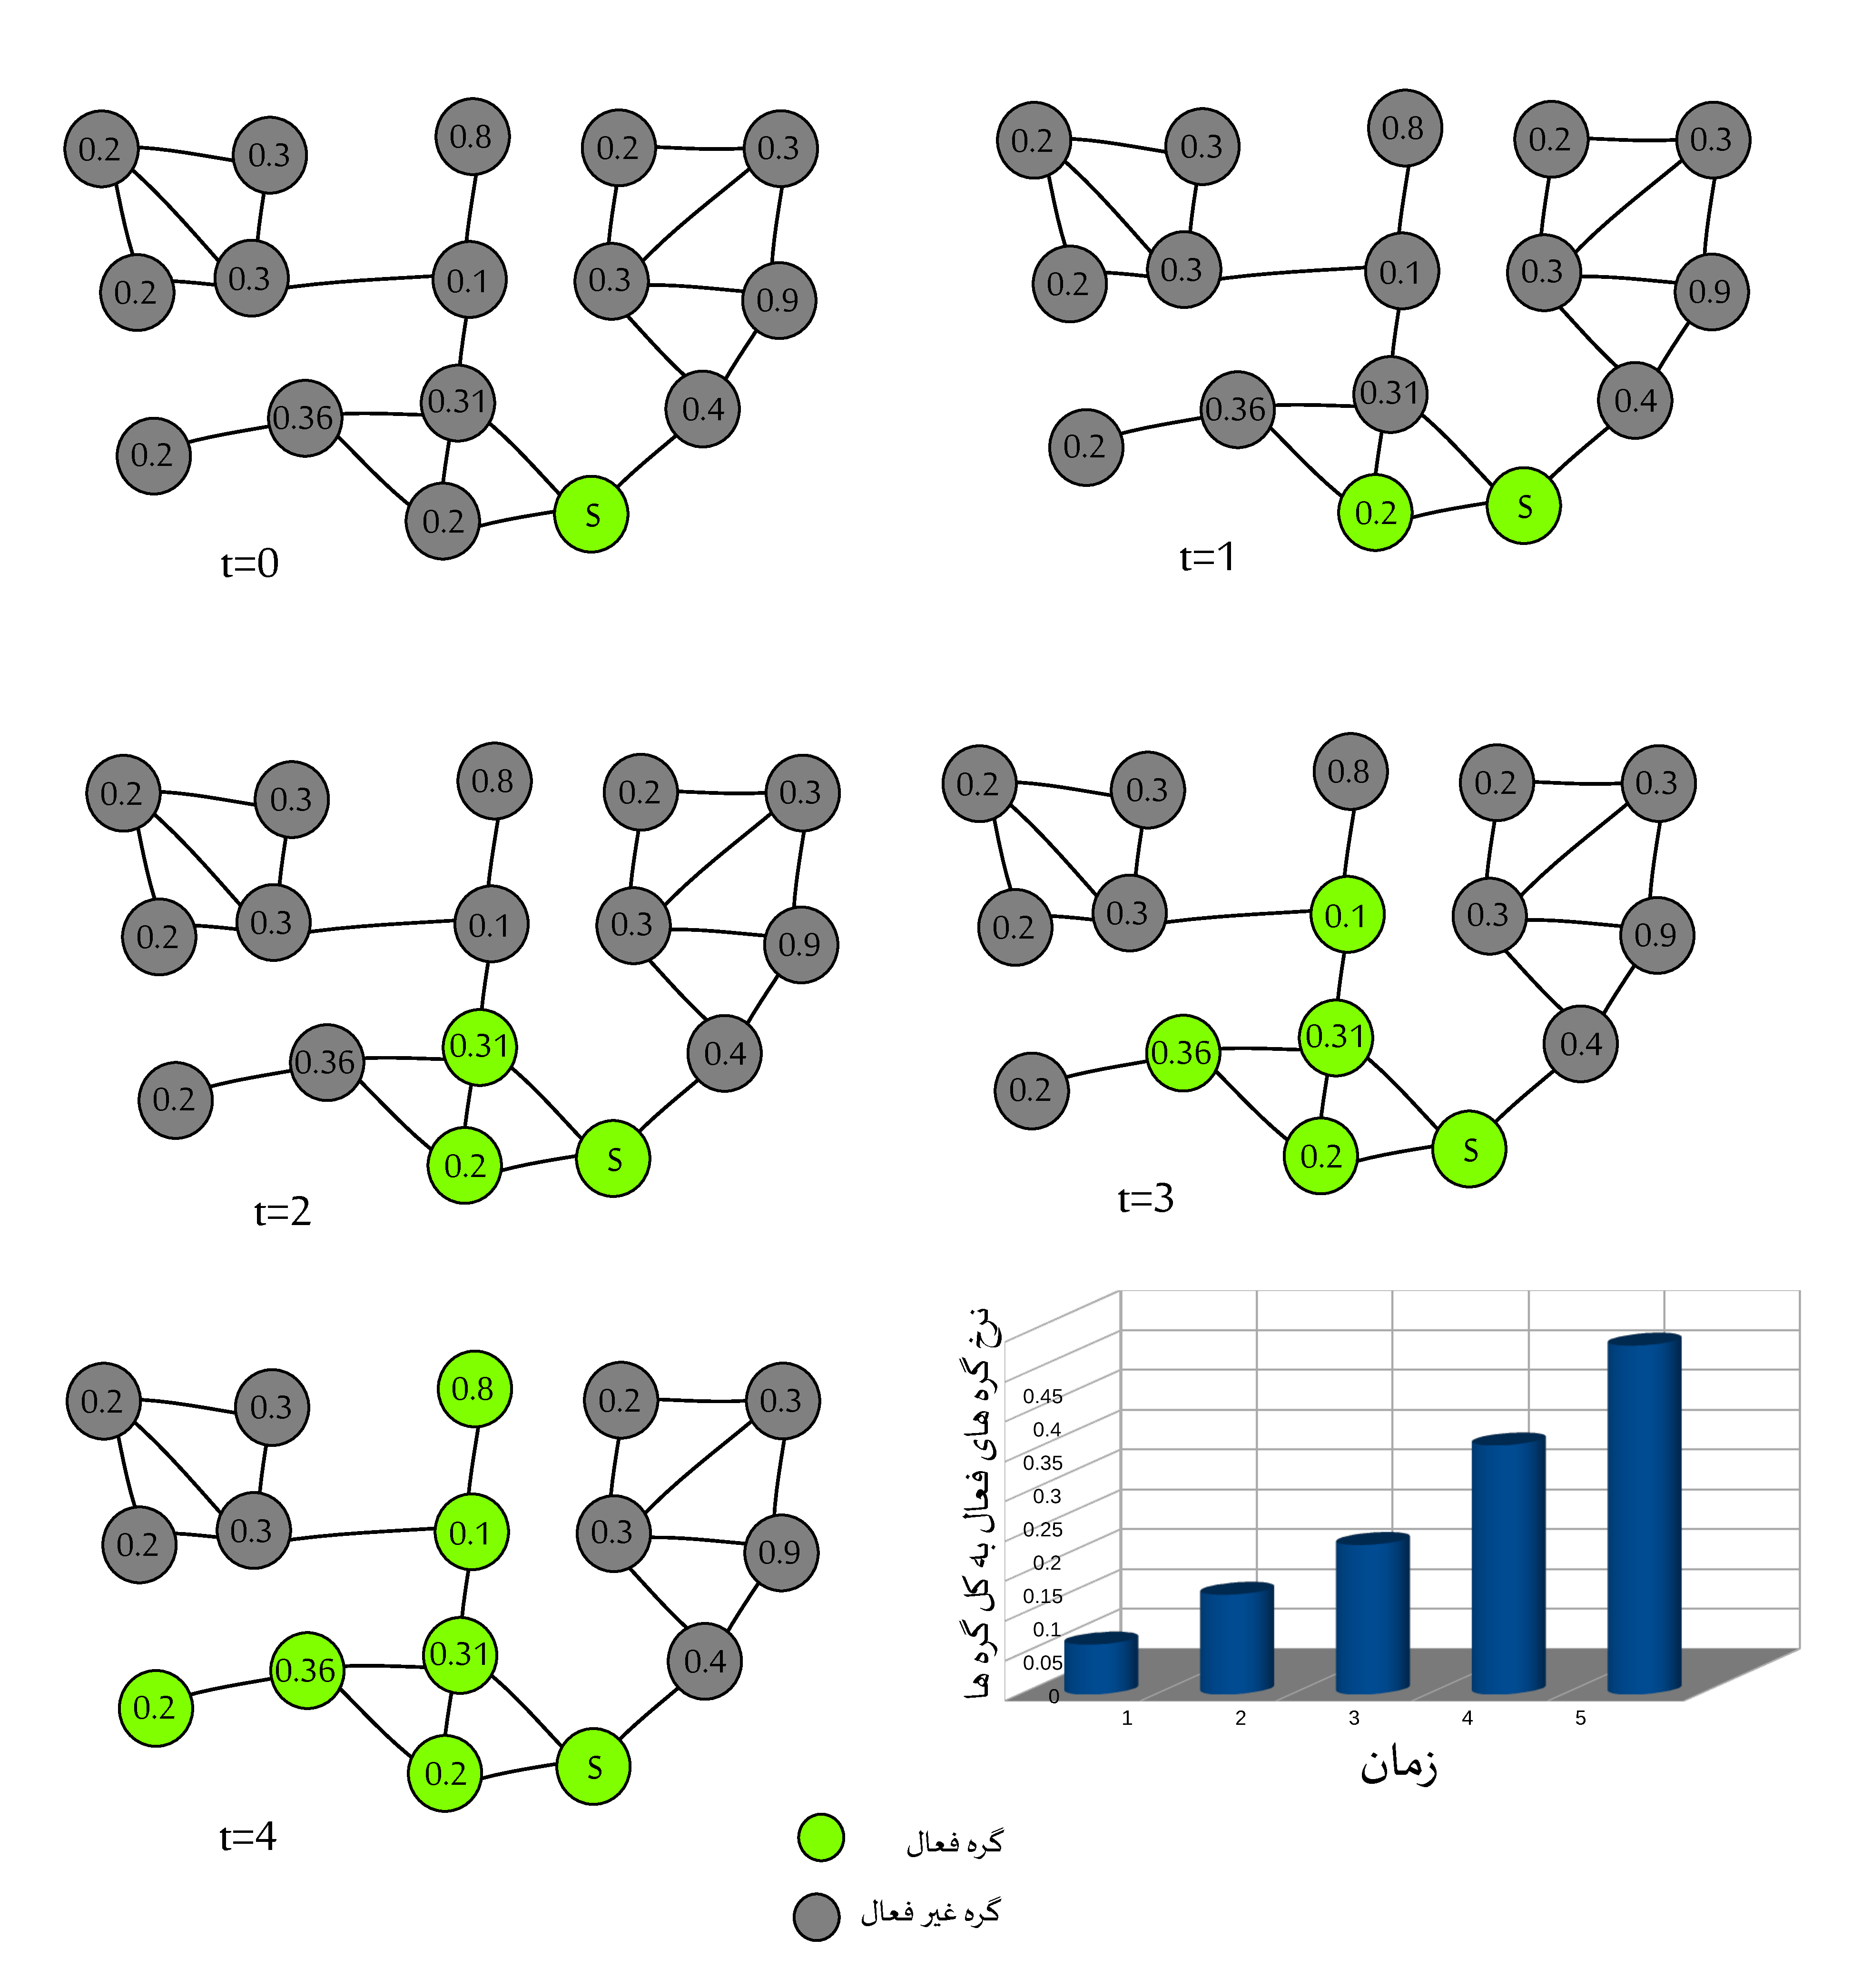
\includegraphics[scale=0.242]{figures/ltm}
 \caption[مدل آستانه خطی]
 { شبیه سازی فرایند کار مدل آستانه خطی با گره \lr{S} به عنوان گره فعال اولیه.}
\end{figure}

\subsection{مدل آستانه اکثریت}
\noindent{
 مدل آستانه اکثریت \پانویس { Majority Threshold Model} یکی از مدل‌های خانواده‌ی آستانه می‌باشد \cite{bhagat_maximizing_2012,richardson_mining_2002,rozin_negativity_2001} که به شدت مورد مطالعه قرار گرفته است. در این مدل گره $v \in V$ وقتی که آستانه $\phi_{v}={(1/2)}d(v)$ به دست بیاید فعال می‌شود \cite{wu_opportunistic_2014}. یکی از کاربرد‌های مهم این مدل در بررسی فرایند نظرسنجی‌هاست. سختی محاسباتی یافتن گره‌های اولیه‌ای که باعث حداکثر شدن گره‌های فعال شده در پایان اجرای این فرایند می‌شوند با سخطی مدل آستانه خطی برابر است.
}

\subsection{مدل آستانه کوچک}
\noindent{
 مدل آستانه کوچک \پانویس { Small Threshold Model} یکی دیگر از مدل‌های خانواده‌ی آستانه می‌باشد \cite{eiselt_competitive_1989,wu_opportunistic_2014} که در این مدل به همگی گره‌های $v \in V$ یک عدد ثابت کوچک $(\phi_v)$ به عنوان آستانه فعال سازی منتسب می‌شود. در \cite{kempe_maximizing_2003} اثبات شده است که برای $\phi_v \geqslant 3 $ مشکل یافتن گره‌های آغازین حداکثرکننده‌ی امر پخش در پایان اجرای این مدل \lr{NP-Hard} است.
}

\subsection{مدل آستانه توافق همگانی}
\noindent{
 در مدل آستانه توافق همگانی\پانویس { Unanimous Threshold Model} آستانه فعال سازی هر گره $v$ به صورت $\phi_v = d(v)$ تعیین می‌شود که $d(v)$ تعداد همسایگان گره $v$ را نشان می‌دهد. این مدل بیشترین مقاومت را نسبت به پخش تاثیر در سطح شبکه اجتماعی دارد. این مدل بیشتر برای بررسی نقاط ضعف امنیتی و بررسی امنیت شبکه‌ها به کار برده می‌شود. برای مثال یک شبکه‌ی اجتماعی را می‌توان درنظر گرفت که در حالت ایده آل یک شایعه وقتی مورد قبول فرد قرار می‌گیرد که مورد قبول همه‌ی همسایگان وی قرار گرفته باشد. یافتن بهترین مجموعه گره‌های نخستین برای بیشینه کردن انتشار در این روش نیز \lr{NP-Hard} است.
}

\subsection{دیگر انواع مدل‌های خانواده‌ی مدل‌های آستانه}
\noindent{
مدل‌های آستانه دیگر به جز موارد ذکر شده‌ی بالا را می‌توان با تعیین تابع آستانه‌ی مناسب طراحی نمود. برای نمونه می‌توان به مدل‌هایی مثل مدل آستانه‌ی خطی رنگی و مدل آستانه جدا \cite{wu_opportunistic_2014,chaintreau_impact_2007,chen_efficient_2009} و همین طور مدل آستانه‌ی متناسب با وزن اشاره نمود. ضمنا در \cite{kempe_maximizing_2003} ثابت شده است که دو مدل انتشار مستقل و آستانه‌ی خطی از نظر ریاضی معادل هم می‌باشند.
}

%\newpage
\section{مدل‌های همه‌گیری}
\noindent
{
در این بخش به معرفی و تشریح مدل‌های همه‌گیری که برای مدل‌کردن فرایند پخش اطلاعات ارایه شده اند می‌پردازیم. 
}
\subsection{مدل \texorpdfstring{\lr{SIR}}{SIR}}
\noindent{
مدل \lr{SIR}\پانویس{ \lr{ Susceptible-Infectious-Recovered}} اولین بار در \cite{m1925applications,kermack1932contributions} برای مدل‌کردن فرایند همه‌گیری بیماری‌های مسری به زبان ریاضی و تحلیلی مطرح شده است. در این مدل در ابتدا یک جمعیت ثابت اولیه به نام $\Omega$ به اندازه‌ی $N$ در نظر گرفته می‌شود. سپس سه مجموعه‌ی $S$ و $I$ و $R$ که به ترتیب نشان دهنده‌ی افراد سالم و مبتلا و افراد درمان‌یافته‌ی(و یا تلف‌شده) $\Omega$ می‌شوند را می‌سازیم. در این مدل اعضای $S$ با نرخ $\alpha$(نرخ ابتلا) به مجموعه‌ی $I$ وارد می‌شوند. هم‌چنین اعضای $I$ هم با نرخ 
$\gamma$ که زمان متوسط دوره‌ی مریضی را نشان می‌دهد، به مجموعه‌ی $R$ وارد می‌شوند. 
\\
\\
\centerline{
\scalebox{1.25}{
\begin{latin}
${\color{blue}{\mathcal{S} \xrightarrow{\alpha} \mathcal{I} \xrightarrow{\gamma } \mathcal{R}}}$
\end{latin}}}

%\\
برای اینکه بتوانیم در لحظه‌ی دلخواه $t$ مقادیر $S(t)$ و $I(t)$ و $R(t)$، که به ترتیب نشان دهنده‌ی تعداد اعضای مجموع‌های $S$ و $I$ و $R$ می‌باشند، محاسبه کنیم نیازمند حل معادله‌های زیر می‌باشیم.
\\
\begin{center}
%\scalebox{1.25}
 {
$\frac{dS}{dt} = - \alpha SI$} %+ \mu (N - S) + \gamma I
\\
%\scalebox{1.25}
 {
$\frac{dI}{dt} = \alpha SI - \gamma I$} %- \mu I 
\\
%\scalebox{1.25}
 {
$\frac{dR}{dt} = \gamma I$ %- \mu I
} 
\end{center}
%%\\
این مدل دارای چند فرض اصلی درباره‌ی روند انتشار بیمارست. برای نمونه در این مدل این فرض وجود دارد که نرخ ابتلا(شتاب پخش‌شدن) برای تمام جمعیت یکسان و برابر $\alpha$ می‌باشد. ضمنا در هر واحد زمان هرکدام از اعضای $S$ بااحتمال برابر به مجموعه‌ی $I$ می‌رود. در این مدل در آستانه‌ی بازتولید(ابتلا و شفا) به نام $\lambda$ وجود برابر 
$\lambda = {\frac{S\alpha}{\gamma}}$
می باشد. طی این رابطه وقتی در این مدل 
$\lambda < 1$ 
باشد مریضی همگیر نخواهد بود و در ابتدا انتشار آن متوقف می‌شود. و اگر 
$\lambda > 1$ 
باشد بیماری به مرور زمان همه‌ی اعضای $S$ را مبتلا خواهد نمود. و هنگامی که 
$\lambda = 1$
باشد سیستم در حال تعادل است ولی در مرز شیوع قرار دارد.

 \begin{figure}[H]
 \centering
 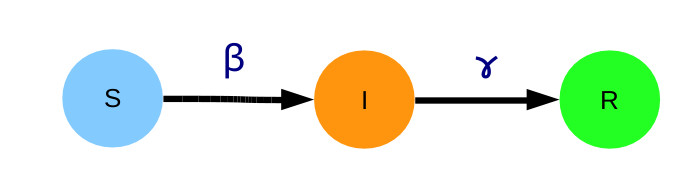
\includegraphics[scale=0.5]{figures/SIR}
 \caption[مدل \texorpdfstring{\lr{SIR}}{SIR}]
 {نمودار تعداد اعضای مجموعه‌های $S$(آبی/صاف) و $I$(سبز/خط تیره) و $R$(قرمز/خط مربع) نسبت به زمان در شبیه‌سازی مدل \lr{SIR} با جمعیت 1000.}
\end{figure}

فقط باید بدین نکته توجه داشت که در همگی مدل‌های ریاضی ارایه شده برای همه‌گیری به صورت کلی فرض بر این گذاشته شده است که $S(t) + I(t) + R(t) = N$ می‌باشد. البته در صورت حذف و یا اضافه شدن یکی از مجموعه‌های سمت چپ معادله تابع مقدار لحظه‌ای مناسب آن مجموعه هم باید حذف و یا اضافه گردد.
}


\subsection{مدل \texorpdfstring{\lr{SI}}{SI}}
\noindent{
این مدل شبیه مدل \lr{SIR} می‌باشد با این تفاوت که در این مدل فرض بر این گذاشته می‌شود که بیماری در حال همه‌گیری درمان ناپذیر است، و یا تاثیر تکنولوژی و یا خبر که در حال انتشار در جامعه می‌باشد کم ناشدنیست. برای نمونه این مدل برای توصیف فرایند شیوع بیماری ایدز و یا چگونگی روند استفاده از تلفن، اینترنت توسط مردم کاربرد دارد. 
\\
\\
\centerline{
\scalebox{1.25}{
\begin{latin}
${\color{blue}{\mathcal{S} \xrightarrow{\alpha} \mathcal{I}}}$
\end{latin}}}

معادله‌های دیفرانسیل این مدل برای محاسبه‌ی $S(t)$ و $I(t)$ در این مدل به صورت زیر خواهند بود.
\\
\begin{center}
%\scalebox{1.25}
 {
$\frac{dS}{dt} = - \alpha SI$} %+ \mu (N - S) + \gamma I
\\
%\scalebox{1.25}
 {
$\frac{dI}{dt} = \alpha SI$} %- \mu I 
\end{center}

دو معادله‌ی فوق برخلاف اکثر معادلات دیفرانسیل مربوط به خانواده‌ی مدل‌های همه‌گیری حل تحلیلی دارند، که به آن تابع رشد لوژستیک\پانویس{ \lr{ Logestic Growth Function}} می‌گویند. در زیر این تابع را که نشان‌دهنده‌ی تعداد افراد مریض جامعه می‌باشد دیده می‌شود.

% \begin{figure}[h]{0.5\textwidth}
% 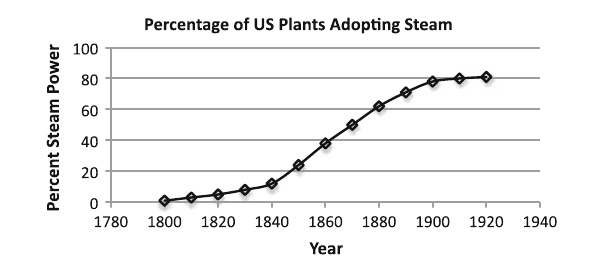
\includegraphics[width=\textwidth]{figures/SI/WaterPower}
% \caption{رشد استفاده‌ی موتور بخار در آمریکا \lr{SI}}
% \end{figure}

\begin{center}
%\scalebox{1.25}
 {
$I(t) = \frac{N I_{0}e^{\alpha t}}{N + I_{0}(e^{\alpha t} - 1)}$
\\
$I_{0}$ نشان دهنده‌ی تعداد افراد مبتلا در لحظه‌ی آغاز است. 
با فرض 
$i_{0}=\frac{I_{0}}{N}$ خواهیم داشت: \\
$i(t) = \frac{i_{0}e^{\alpha t}}{1 + Ii_{0}(e^{\alpha t} - 1)}$}
\\
\end{center}

\begin{figure}[h]
 \centering
 \begin{subfigure}[b]{0.6\textwidth}
 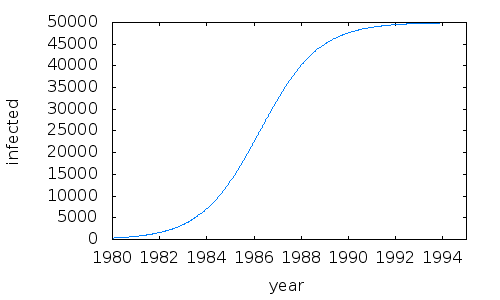
\includegraphics[width=\textwidth]{figures/SI/aids1980-95}
 \caption{رشد مبتلایان به ایدز از سال ۱۹۸۰ تا ۱۹۹۵ در آمریکا.}
 \end{subfigure}%
 
 %add desired spacing between images, e. g. ~, \quad, \qquad, \hfill etc.
 %(or a blank line to force the subfigure onto a new line)
 \begin{subfigure}[b]{0.6\textwidth}
 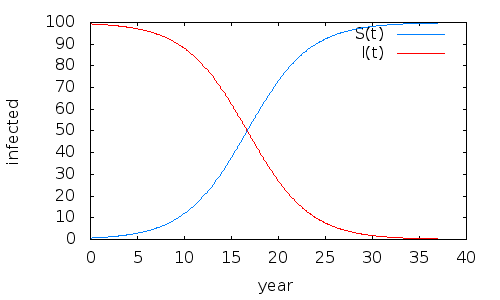
\includegraphics[width=\textwidth]{figures/SI/aidsSt-It}
 \caption{شبیه سازی مدل \lr{SI}}
 \end{subfigure}
 
 \caption[شبیه‌سازی مدل \texorpdfstring{\lr{SI}}{SI}]
 {شبیه‌سازی همه‌گیری به کمک مدل \lr{SI} با تابع رشد لوژستیک 
 $\frac{50000}{1+e^{5+(-0.8)x}}$.}
\end{figure}
}

\subsection{مدل \texorpdfstring{\lr{SIS}}{SIS}}
\noindent{
این مدل بسیار شبیه مدل \lr{SIR} می‌باشد با این تفاوت که در این مدل فرض بر این گذاشته می‌شود که بیماران(اعضای $I$) بعد از گذراندن بیماری شفا می‌یابند و به مجموعه‌ی $S$ بر‌می‌گردند. به زبان ساده در این مدل پس از ابتلا بعد از مدتی عضو بیمار دوباره به اجتماع افراد سالم مستعد بیماری باز می‌گردد.
\\
\\
\centerline{
\scalebox{1.25}{
\begin{latin}
${\color{blue}{\mathcal{S} \xrightarrow{\alpha} \mathcal{I} \xrightarrow{\gamma } \mathcal{S}}}$
\end{latin}}}

معادله‌های دیفرانسیل این مدل برای محاسبه‌ی $S(t)$ و $I(t)$ به صورت زیر خواهند بود.
\\
\begin{center}
%\scalebox{1.25}
 {
$\frac{dS}{dt} = - \alpha SI + \gamma I$} %+ \mu (N - S) + \gamma I
\\
%\scalebox{1.25}
 {
$\frac{dI}{dt} = \alpha SI - \gamma I$} %- \mu I 
\end{center}

}

یک تفاوت عمده‌ی این مدل با مدل \lr{SIR} و \lr{SI} در امکان از بین نرفتن بیماری و یا عامل‌ همه‌گیر در یک جامعه‌ می‌باشد. به زبان ساده‌تر چرخه ابتلا و شفا می‌تواند تا ابد در جامعه تکرار شود.

\subsection{مدل \texorpdfstring{\lr{SIRS}}{SIRS}}
\noindent{
این مدل هم بسیار شبیه مدل $SIR$ می‌باشد با این تفاوت که اعضای مجموعه‌ی $R$ بعد از مدتی به مجموعه‌ی $S$ می‌پیوندند.
\\
\\
\centerline{
\scalebox{1.25}{
\begin{latin}
${\color{blue}{\mathcal{S} \xrightarrow{\alpha} \mathcal{I} \xrightarrow{\gamma } \mathcal{R}} \xrightarrow{\frac{1}{\sigma}} \mathcal{S}}$
\end{latin}}}

معادله‌های دیفرانسیل این مدل برای محاسبه‌ی مقادیر $S(t)$ و $I(t)$ و $R(t)$، به صورت زیر خواهند بود.

\begin{center}
%\scalebox{1.25}
 {
$\frac{dS}{dt} = - \alpha SI + \sigma R$}
\\
%\scalebox{1.25}
 {
$\frac{dI}{dt} = \alpha SI - \gamma I$} 
\\
%\scalebox{1.25}
 {
$\frac{dR}{dt} = \gamma I - \sigma R$}

\end{center}

}

\subsection{دیگر مدل‌های همه‌گیری}
\noindent{
مشتقات زیادی از مدل \lr{SIR} برای مدل‌سازی فرایند همه‌گیری و پخش بیماری و همین‌طور انتشار شایعه در سطح جوامع انسانی مطرح شده است. برای مثال به‌جز مدل‌های همه‌گیری ذکر‌شده تا به الآن در این نوشته، مدل‌های \lr{SEIS} و \lr{SEIR} و \lr{MSIR} و \lr{MSEIR} و \lr{MSEIRS} و \lr{SEIZ} \cite{hethcote2000mathematics} که همگی جزو مدل‌های احتمالی همه‌گیری می‌باشند، نیز برای مدل‌سازی پخش اطلاعات به ‌کار رفته اند. در مدل‌های فوق الذکر حرف \lr{M}\پانویس{ \lr{Maternally-derived immunity}} نشاندهنده‌ی حالتی است که فرد در ابتدا برای مدتی دارای مصونیت به عامل همه‌گیری است. حروف \lr{E}\پانویس{ \lr{Exposed}} و \lr{Z}\پانویس{ \lr{Maternally-derived immunity}} هم به ترتیب معنای حالت‌های نهفتگی بیماری و حالت شک به صحت اطلاعات از جانب فرد مطلع(این مدل درباره‌ی مدل‌سازی شایعه کاربرد دارد) می‌باشند. 
}

\begin{figure}[h]
 \centering
 \begin{subfigure}[b]{0.32\textwidth}
 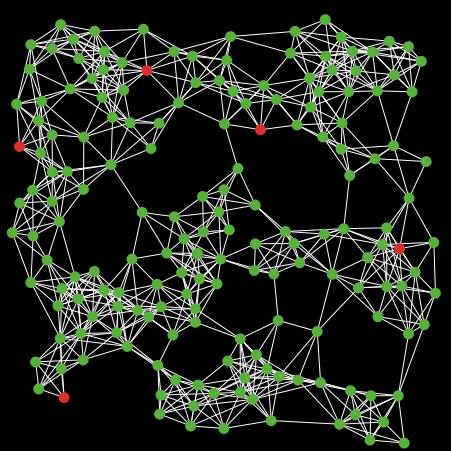
\includegraphics[width=\textwidth]{figures/SIRS/t0}
 \caption{وضعیت جامعه در $t=0$}
 
 \end{subfigure}%
 ~ %add desired spacing between images, e. g. ~, \quad, \qquad, \hfill etc.
 %(or a blank line to force the subfigure onto a new line)
 \begin{subfigure}[b]{0.32\textwidth}
 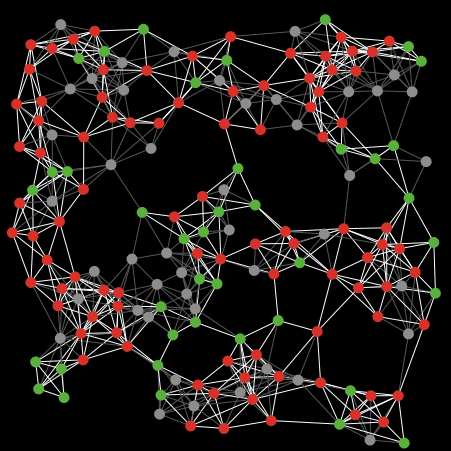
\includegraphics[width=\textwidth]{figures/SIRS/t223}
 \caption{وضعیت جامعه در $t=223$}
 
 \end{subfigure}
 ~ %add desired spacing between images, e. g. ~, \quad, \qquad, \hfill etc.
 %(or a blank line to force the subfigure onto a new line)
 \begin{subfigure}[b]{0.32\textwidth}
 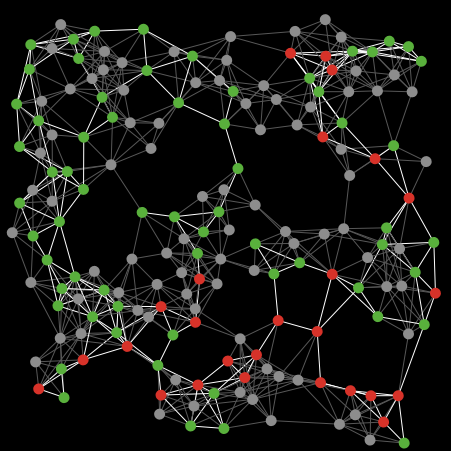
\includegraphics[width=\textwidth]{figures/SIRS/t540}
 \caption{وضعیت جامعه در $t=540$}
 %\label{fig:mouse}
 \end{subfigure}
 ~ %add desired spacing between images, e. g. ~, \quad, \qquad, \hfill etc.
 %(or a blank line to force the subfigure onto a new line)
 
 
 \begin{subfigure}[b]{0.4\textwidth}
 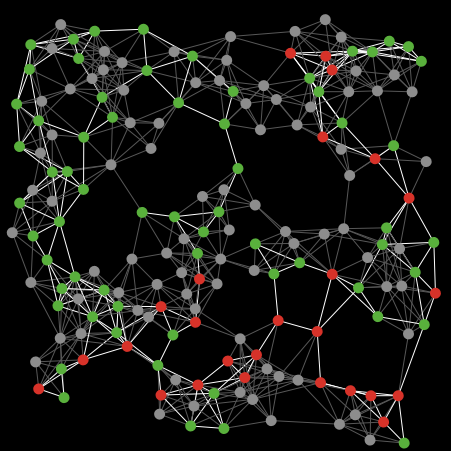
\includegraphics[width=\textwidth]{figures/SIRS/t540}
 \caption{وضعیت جامعه در پایان شبیه‌سازی}
 
 \end{subfigure}
 ~~~
 \begin{subfigure}[b]{0.35\textwidth}
 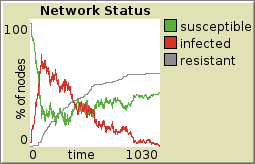
\includegraphics[width=\textwidth]{figures/SIRS/SIRS}
 \caption{نمودار وضعیت جامعه در طی شبیه‌سازی}
 
 \end{subfigure}
 \caption[شبیه‌سازی مدل \texorpdfstring{\lr{SIRS}}{SIRS}]{شبیه‌سازی همه‌گیری به کمک مدل \lr{SIRS} با $\alpha=0.025$ و ${\frac{1}{\sigma}} ={\gamma}=0.05.$ و $N=175$.
 (رنگ قرمز و سبز و خاکستری به ترتیب افراد بیمار و سالم و افراد شفا ‌یافته‌ی جامعه را نشان می‌دهند.)}
\end{figure}

\section{مدل‌های دیگر پخش اطلاعات}
\noindent{
جدا از سه دسته مدل مطرح که گفته شد مدل‌های دیگری هم برای مدل‌کردن فرایند پخش اطلاعات ارایه شده اند
\cite{kwon_information_2009,hajibagheri_modeling_2013,broecheler_scalable_2010,kim_modeling_2011,sotoodeh_general_2013,he_influence_2012,jiang_modeling_2014,snijders_introduction_2010,hurd_watts_2013,wang_modeling_2013,lande_model_2008,lou_social_2014,lou_modeling_2014,cheng_epidemic_2013}.
اکثر این مدل‌ها از مدل‌های گفته شده قبلی مشتق شده اند. البته مدل‌های دیگری نیز برای امر پخش در سطح شبکه‌های پیچیده ارایه شده اند، مانند \cite{lin_modelling_2014} که مسئله‌ی پخش با چند منبع را به صورت خاص مورد مطالعه قرار داده اند. 

}

 \begin{figure}[H]
 \centering
 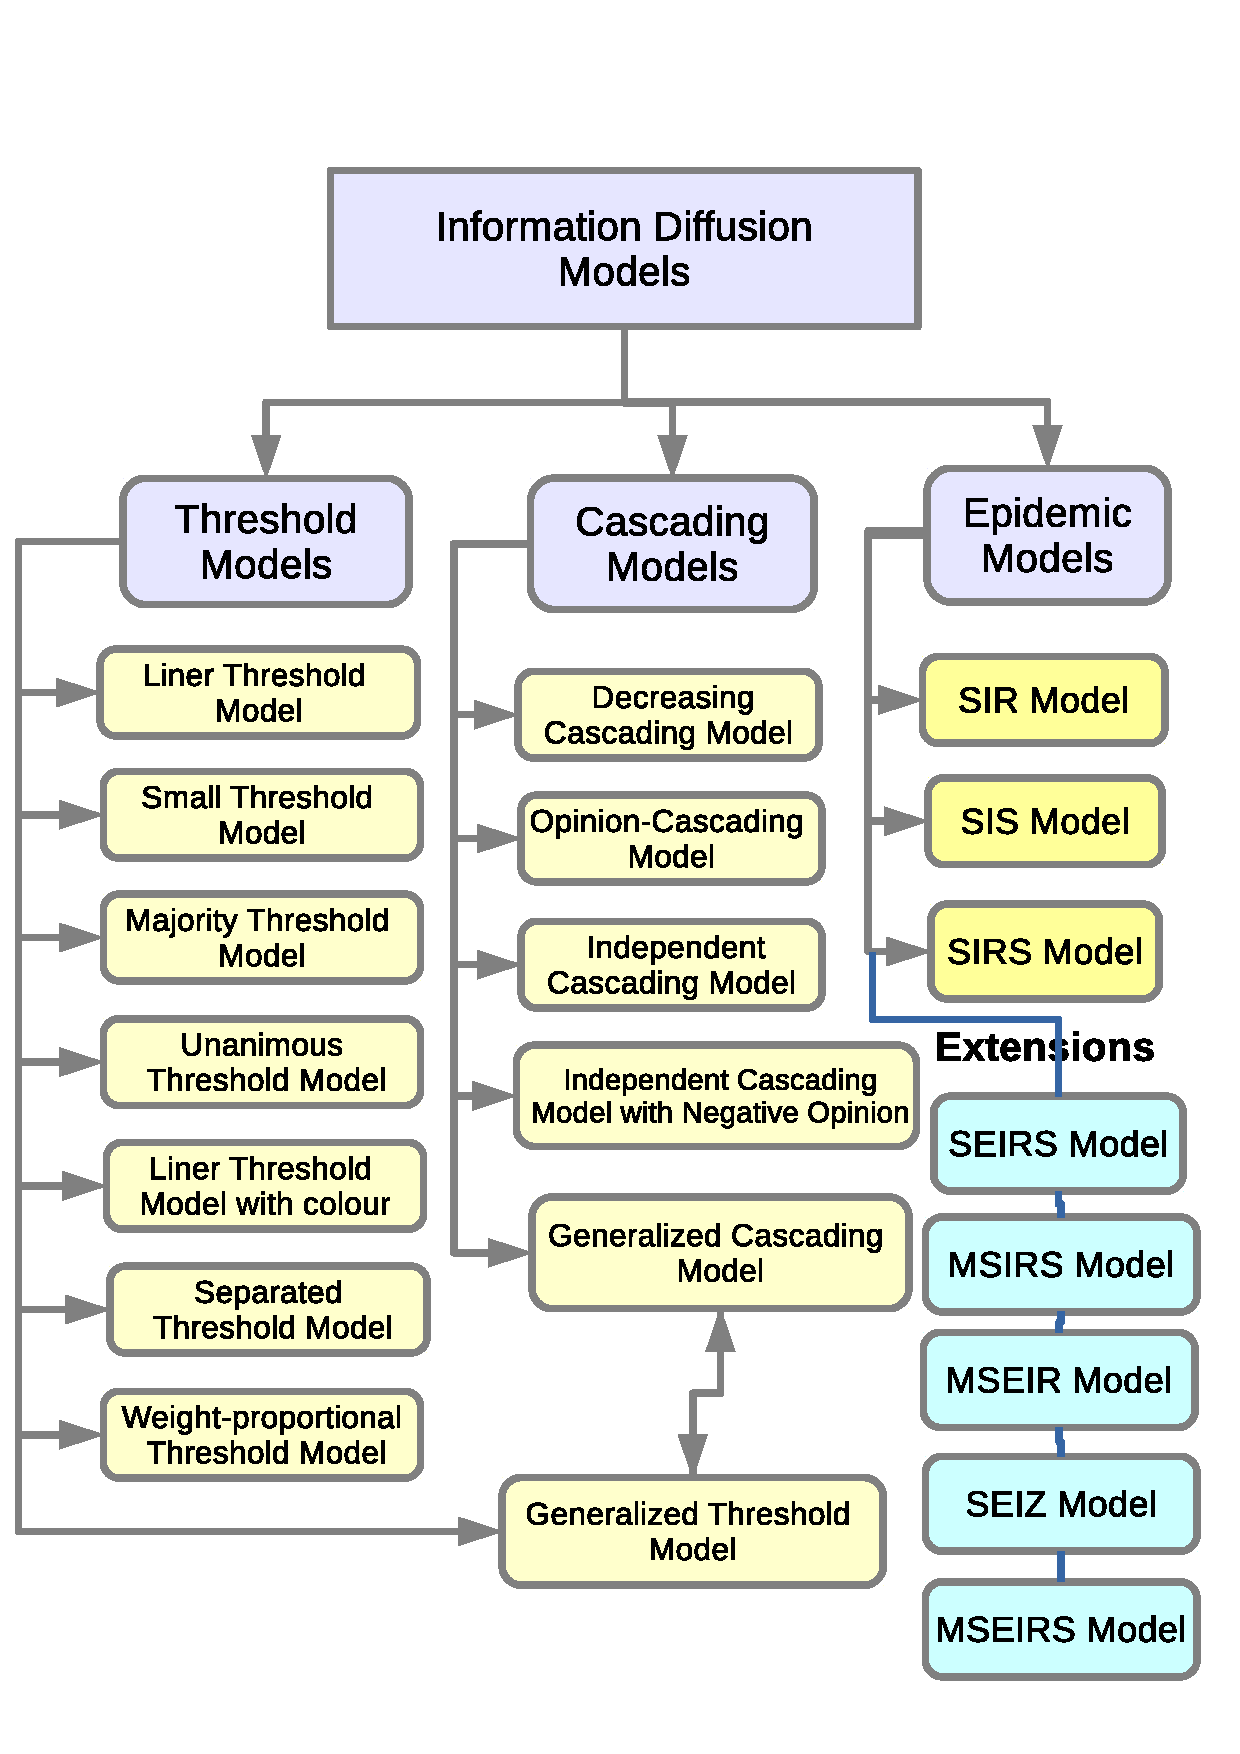
\includegraphics[scale=0.6]{figures/IDMO}
 \caption[مدل‌های اصلی پخش اطلاعات]
 {نمایی کلی از خانواده مدل‌های اصلی پخش اطلاعات.}
\end{figure}

\section{خلاصه‌ی مطالب فصل}
\noindent{
در این فصل سه گروه اصلی از مدل‌های پخش اطلاعات معرفی شدند. سه خانواده‌ی معرفی شده شامل مدل‌های آستانه و انتشار و همه‌گیری بیماری می‌باشند. مدل‌های \lr{LT} و \lr{IC} بسیار محبوب محققان برای مد‌سازی فرایند پخش اطلاعات می‌باشند و در ابتدا برای یافتن روشی الگوریتمیک برای به حداکثر رساندن تاثیر اجتماعی مطرح شدند. یافتن $k$ گره‌ای که فرایند پخش را حداکثر کنند در این مدل از نظر محاسباتی جزو دسته مسائل \lr{NP-Hard} می‌باشد، لذا الگوریتم‌های هیوریستیک زیادی برای این دو مدل مانند الگوریتم‌های \lr{CELF} و \lr{CELF++} و \lr{SIMPATH} \cite{kempe_maximizing_2003,chen_scalable_2010,lv_improved_2014,goyal_simpath:_2011} تا به امروز ارایه شده اند.
\\
\indent
مدل‌های همه‌گیری مطرح و مورد استفاده هم مانند \lr{SIR} و \lr{SIRS} و \lr{SIS} در این فصل توضیح داده شدند. پخش اطلاعات دارای شباهت‌های زیادی با فرایند همه‌گیری بیماری‌ دارد، به طوری که مدل‌های همه‌گیری فوق الذکر در اکثر موارد توانسته اند برآورد درستی نسبت به روند واقعی فرایند پخش 
اطلاعات به دست بدهند.

}
\end{persian}